\subsection{Process View}

\copied{Process view : The process view deals with the dynamic aspects of the system, explains the system processes and how they communicate, and focuses on the runtime behavior of the system. The process view addresses concurrency, distribution, integrators, performance, and scalability, etc. UML Diagrams to represent process view include the Activity diagram.}
{from wikipedia}
This view mainly discuss about runtime, concurrency, communication, and synchronization of the process running in the system. \\

The program flow and business logic of the system are captured in this section with the aid of several activity diagrams.

\subsubsection*{Flood monitoring}

The activity diagram in figure~\ref{fig:activity-monitoring} shows the flow of the flood monitoring process.


\begin{figure}[h]
\centering
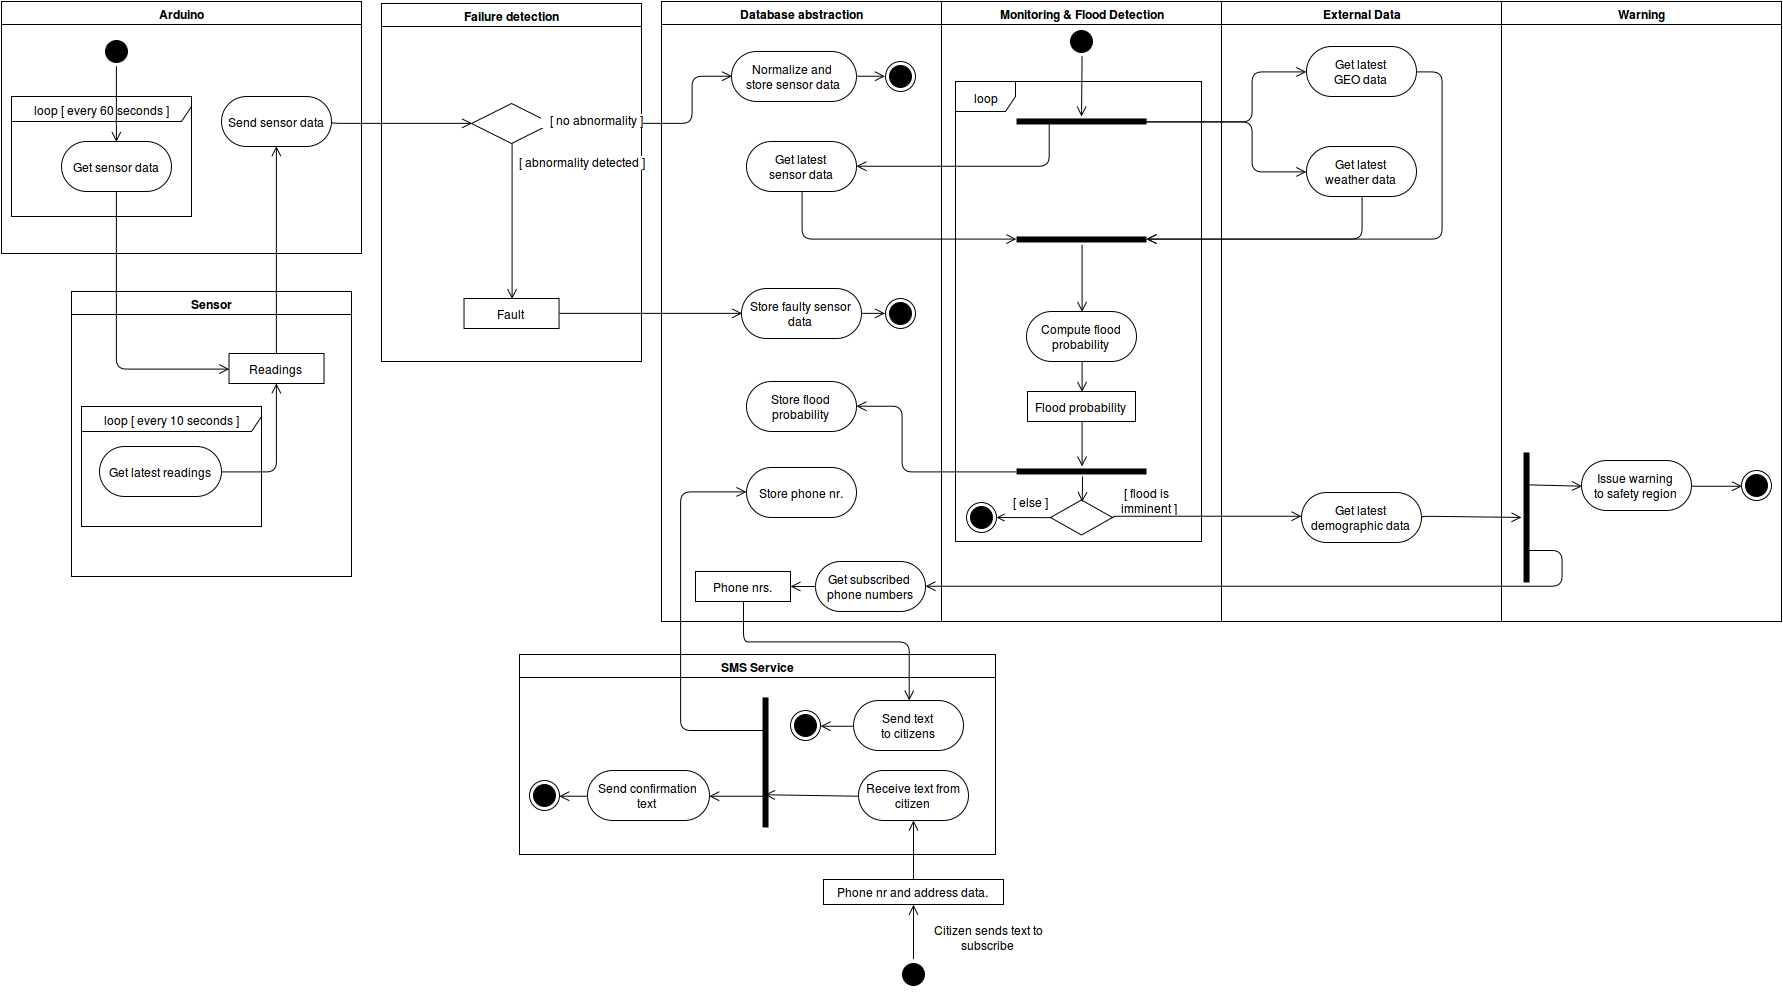
\includegraphics[keepaspectratio=true,width=1.0\textwidth]{{\viewimages/activity_monitoring}.png}
\caption{An activity diagram of the flood monitoring process}
\label{fig:activity-monitoring}
\end{figure}


\subsubsection*{Sending warnings}

In figure~\ref{fig:warning} a sequence diagram of sending warnings to the emergency room and citizens can be seen. The sequence diagram contains a time constraint of 10 seconds and 5 minutes, for warning the emergency room and all citizens respectively.

\begin{figure}[h]
\centering
\includegraphics[keepaspectratio=true,width=1.0\textwidth]{{\viewimages/sequence_warning}.png}
\caption{A sequence diagram of sending warnings to citizens and emergency room}
\label{fig:warning}
\end{figure}


\subsubsection*{Sending the sensor data}
In figure~\ref{fig:sequence-sensordata} a sequence diagram of sending the sensor data can be seen. The sensor has two running threads: one reading the measurements and the other for sending the data every 60 seconds.

\begin{figure}[h]
\centering
\includegraphics[keepaspectratio=true,width=0.7\textwidth]{{\viewimages/sequence_sensor}.png}
\caption{An activity diagram of the flood monitoring process}
\label{fig:sequence-sensordata}
\end{figure}